
\documentclass[12pt,a4paper]{article}

\usepackage[T1]{fontenc}
\usepackage[utf8]{inputenc}
\usepackage[romanian]{babel}
\usepackage{lmodern}
\usepackage{geometry}
\usepackage{graphicx}
\usepackage{amsmath}
\usepackage{enumitem}
\usepackage{listings}

\geometry{margin=2.5cm}
\setlength{\parindent}{0pt}
\setlength{\parskip}{8pt}

\begin{document}

\begin{titlepage}
\begin{center}

{\Large Universitatea „Alexandru Ioan Cuza” din Iași}

\vspace{0.4cm}

{\Large Facultatea de Informatică}

\vspace{3cm}

{\LARGE\textbf{Tehnici de Programare Multiprocesor}}

\vspace{1cm}

{\Huge\textbf{TEMA TPM}}

\vspace{3cm}

{\large
\begin{tabular}{ll}
Motricală Alin-Gabriel & Grupa 3A4\\[0.3cm]
Gabriela Țibuleac & Grupa 3E3
\end{tabular}
}

\vspace{1cm}

{\large Seria A}

\vfill

{\large Iași, 2026}

\end{center}
\end{titlepage}


\section*{Exercițiul 1}

\begin{center}
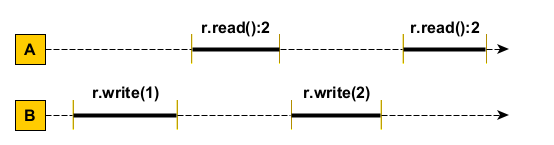
\includegraphics[width=0.95\textwidth]{imagini/ex1.png}
\end{center}

\subsection*{a) Linearizabilitate}

Istoria \textbf{nu este linearizabilă}.

Pentru ca o istorie să fie linearizabilă,
fiecare operație trebuie să aibă un punct
de linearizare între începutul și sfârșitul
execuției sale. În plus, trebuie respectată
ordinea temporală a operațiilor care nu
se suprapun.

În diagrama dată, threadul B execută mai întâi
operația $r.write(1)$, după care threadul A
execută o citire care returnează valoarea 2.

Observăm că prima operație $r.read()$
se termină înainte să înceapă $r.write(2)$.

Astfel, prima citire nu poate returna valoarea
2, deoarece această valoare nu a fost încă
scrisă în registru.

Valoarea inițială a registrului este 0,
iar singura scriere finalizată înaintea
primei citiri este $r.write(1)$.

Prin urmare, prima citire ar trebui să
returneze valoarea 1.

Nu există un punct de linearizare valid
care să justifice prima citire cu valoarea 2,
fără să încălcăm ordinea temporală reală.

În concluzie, \textbf{istoria nu este linearizabilă}.

\subsection*{b) Consistență secvențială}

Istoria \textbf{este consistentă secvențial}.

Consistența secvențială presupune că putem
găsi o ordine secvențială a tuturor
operațiilor, astfel încât să respectăm
ordinea operațiilor din fiecare thread
și să obținem aceleași rezultate.

Spre deosebire de linearizabilitate,
nu trebuie păstrată ordinea temporală
dintre threaduri diferite.

În cazul nostru, threadul B execută
două scrieri, în ordinea $r.write(1)$
și $r.write(2)$.

Threadul A execută două citiri,
ambele returnând valoarea 2.

Putem construi următoarea ordine:

\[
\begin{aligned}
&B:r.write(1)\\
&\downarrow\\
&B:r.write(2)\\
&\downarrow\\
&A:r.read() = 2\\
&\downarrow\\
&A:r.read() = 2
\end{aligned}
\]

Această ordine este validă deoarece:

\begin{itemize}
    \item Threadul B păstrează ordinea
    celor două scrieri.
    \item Threadul A păstrează ordinea
    celor două citiri.
    \item Ambele citiri returnează 2,
    deoarece sunt plasate după
    operația $r.write(2)$.
\end{itemize}

Chiar dacă în execuția reală prima citire
se termină înainte de începerea celei
de-a doua scrieri, consistența secvențială
permite această reordonare între threaduri.

Prin urmare, \textbf{istoria este
consistentă secvențial}.

\newpage
\section*{Exercițiul 2}

În implementarea dată există câteva probleme
legate de inițializarea threadului, vizibilitatea
variabilelor și utilizarea lock-ului.

\subsection*{Probleme identificate}

\begin{enumerate}
    \item \textbf{Constructorul este declarat greșit.}

    Metoda \texttt{MyThread} are tipul de
    returnare \texttt{void}, deci nu este un
    constructor. Pentru a inițializa corect
    obiectul, trebuie eliminat \texttt{void}.

    \item \textbf{Variabila alive nu este volatile.}

    Dacă variabila \texttt{alive} este modificată
    de un alt thread, nu avem garanția că
    modificarea va fi observată imediat.
    Declararea ei ca \texttt{volatile} asigură
    vizibilitatea modificărilor între threaduri.

    \item \textbf{Folosirea incorectă a blocului try-finally.}

    În codul inițial, \texttt{unlock()} este apelat
    în blocul \texttt{finally}, chiar dacă threadul
    nu a reușit să obțină lock-ul.

    De exemplu, dacă \texttt{someNonExclusiveMethod()}
    aruncă o excepție, se ajunge la \texttt{finally}
    fără ca \texttt{lock()} să fi fost apelat.
    Același lucru se poate întâmpla dacă
    \texttt{lock()} eșuează înainte de obținerea
    lock-ului.

    De aceea, metoda neexclusivă se execută
    în afara secțiunii critice, iar apelul
    \texttt{lock()} este mutat înainte de
    \texttt{try}. Blocul \texttt{finally} se
    ocupă astfel doar de eliberarea unui lock
    obținut cu succes.
\end{enumerate}

\subsection*{Varianta corectată}

\begin{lstlisting}[language=Java,
    basicstyle=\ttfamily\small,
    breaklines=true,
    frame=single,
    showstringspaces=false]
public class MyThread extends Thread {
    private final SharedObject sharedObject;
    private final SharedLock sharedLock;
    private volatile boolean alive = true;

    public MyThread(SharedObject sharedObject,
                    SharedLock sharedLock) {
        this.sharedObject = sharedObject;
        this.sharedLock = sharedLock;
    }

    public void stopRunning() {
        alive = false;
    }

    @Override
    public void run() {
        while (alive) {
            sharedObject.someNonExclusiveMethod();

            sharedLock.lock();
            try {
                sharedObject.someExclusiveMethod();
            } finally {
                sharedLock.unlock();
            }
        }
    }
}
\end{lstlisting}

\subsection*{Explicația soluției}

În varianta corectată, constructorul
inițializează obiectele partajate,
iar variabila \texttt{alive} este declarată
\texttt{volatile}, pentru a permite oprirea
threadului din exterior.

Metoda \texttt{someNonExclusiveMethod()}
se execută fără lock, deoarece nu necesită
excludere mutuală.

Înainte de executarea metodei
\texttt{someExclusiveMethod()}, threadul
obține lock-ul prin \texttt{lock()}.

După obținerea lock-ului, folosim
\texttt{try-finally} pentru a garanta
eliberarea acestuia chiar dacă apare
o excepție în secțiunea critică.

Astfel, apelul \texttt{unlock()} se execută
doar după ce lock-ul a fost obținut
cu succes.


\newpage
\section*{Exercițiul 3}

\subsection*{a) ShadyLock -- Starvation-free}

Algoritmul \textbf{nu este starvation-free}.

Un algoritm este starvation-free dacă fiecare
thread care încearcă să obțină lock-ul reușește
în cele din urmă să intre în secțiunea critică,
presupunând că threadurile continuă să execute
instrucțiuni și că secțiunile critice se termină.

În algoritmul dat, variabilele \texttt{turn}
și \texttt{used} sunt partajate între threaduri.
Problema este că instrucțiunile care verifică
și modifică aceste variabile nu formează
o operație atomică.

Putem construi o execuție cu două threaduri,
T1 și T2, având ID-urile 1 și 2.
Inițial, \texttt{used = false}.

\begin{center}
\begin{tabular}{|c|l|l|}
\hline
Pas & Thread & Operație \\ \hline
1 & T1 & turn = 1 \\ \hline
2 & T1 & verifică used = false \\ \hline
3 & T2 & turn = 2 \\ \hline
4 & T2 & verifică used = false \\ \hline
5 & T1 & used = true \\ \hline
6 & T1 & turn != 1, reia bucla \\ \hline
7 & T1 & turn = 1 \\ \hline
8 & T1 & verifică used = true \\ \hline
9 & T2 & used = true \\ \hline
10 & T2 & turn != 2, reia bucla \\ \hline
\end{tabular}
\end{center}

După această execuție, variabila
\texttt{used} rămâne \texttt{true},
dar niciun thread nu a reușit să
termine metoda \texttt{lock()}.

Ambele threaduri rămân în bucla interioară:

\begin{lstlisting}[language=Java]
do {
    turn = me;
} while (used);
\end{lstlisting}

Variabila \texttt{used} poate deveni
\texttt{false} doar prin apelul
\texttt{unlock()}, însă niciun thread
nu a obținut lock-ul și nu poate
ajunge să îl elibereze.

Prin urmare, algoritmul poate ajunge
într-o situație de deadlock.
Aceasta încalcă și proprietatea
starvation-free, deoarece threadurile
pot aștepta la nesfârșit.

\textbf{Concluzie:} Algoritmul ShadyLock
nu este starvation-free.

\subsection*{b) VeryShadyLock -- Excludere mutuală}

Algoritmul \textbf{nu asigură excluderea mutuală}.

Excluderea mutuală presupune că, la un moment
dat, cel mult un thread poate executa
secțiunea critică protejată de lock.

Deși algoritmul folosește un lock intern
care garantează excluderea mutuală,
acesta nu este obținut de toate threadurile.

Mai exact, dacă expresia
\texttt{x != me} este falsă,
threadul poate termina metoda
\texttt{lock()} fără să obțină
lock-ul intern.

Pentru a demonstra problema, considerăm
două threaduri, T1 și T2, cu ID-urile 1 și 2.
Inițial, \texttt{x = 0} și \texttt{y = 0}.

\begin{center}
\begin{tabular}{|c|l|l|}
\hline
Pas & Thread & Operație \\ \hline
1 & T1 & x = 1 \\ \hline
2 & T1 & y == 0, continuă \\ \hline
3 & T2 & x = 2 \\ \hline
4 & T2 & y == 0, continuă \\ \hline
5 & T2 & y = 2 \\ \hline
6 & T2 & x == 2, nu ia lock-ul intern \\ \hline
7 & T2 & Intră în secțiunea critică \\ \hline
8 & T1 & y = 1 \\ \hline
9 & T1 & x != 1 \\ \hline
10 & T1 & Obține lock-ul intern \\ \hline
11 & T1 & Intră în secțiunea critică \\ \hline
\end{tabular}
\end{center}

La pasul 7, T2 intră în secțiunea
critică fără să obțină lock-ul intern.

Ulterior, T1 observă că
\texttt{x != 1}, deci apelează
\texttt{lock.lock()}.

Deoarece T2 nu a obținut lock-ul
intern, acesta este liber,
iar T1 îl poate obține imediat.

Astfel, T1 intră și el în secțiunea
critică, în timp ce T2 se află încă acolo.

Acest lucru este posibil deoarece
verificarea și modificarea variabilei
\texttt{y} nu se realizează atomic.
Ambele threaduri pot observa
\texttt{y = 0} și pot continua.

\textbf{Concluzie:} Algoritmul
VeryShadyLock nu garantează
excluderea mutuală, chiar dacă
lock-ul intern este corect.

\subsection*{c) ShadyChoice}

Trebuie să demonstrăm că, într-o execuție
cu $n > 1$ threaduri:

\begin{itemize}
    \item cel mult un thread poate returna
    valoarea \texttt{red};
    \item cel mult $n-1$ threaduri pot returna
    valoarea \texttt{black}.
\end{itemize}

\subsubsection*{1. Cel mult un thread returnează red}

Un thread poate returna \texttt{red} numai dacă
citește \texttt{getWhite = false}, execută
\texttt{getWhite = true} și apoi găsește
\texttt{last == me}.

Presupunem, prin reducere la absurd, că două
threaduri diferite, T1 și T2, returnează
ambele \texttt{red}.

Notăm cu $W_i(last)$ scrierea ID-ului threadului
Ti în variabila \texttt{last}, iar cu $R_i(last)$
citirea finală a acestei variabile.
În mod asemănător, folosim $R_i(getWhite)$ și
$W_i(getWhite)$ pentru accesările variabilei
\texttt{getWhite}.

Pentru ca ambele threaduri să ajungă la
\texttt{red}, fiecare trebuie să citească
\texttt{getWhite = false} înainte ca celălalt
să scrie \texttt{getWhite = true}.
Deoarece scrierea în \texttt{last} se face înaintea
acestei citiri, avem:

\[
W_1(last) < R_1(getWhite) < W_2(getWhite) < R_2(last)
\]

și, simetric:

\[
W_2(last) < R_2(getWhite) < W_1(getWhite) < R_1(last)
\]

Așadar, scrierile ambelor threaduri în
\texttt{last} au loc înaintea citirilor finale
ale ambelor threaduri.

Dacă T1 scrie ultimul dintre cele două,
valoarea 2 a lui T2 este suprascrisă și T2
nu mai poate citi propriul ID. Dacă T2 scrie
ultimul, T1 nu mai poate citi valoarea 1.
Alte threaduri pot scrie alte ID-uri, dar nu
pot face ca ambele threaduri să-și citească
propriul ID, deoarece ID-urile sunt unice.

În ambele situații, cel puțin unul dintre
threaduri nu poate returna \texttt{red},
contrar presupunerii inițiale.

Prin urmare, \textbf{cel mult un thread poate
returna red}.

\[
\boxed{\text{Numărul de red} \leq 1}
\]

\subsubsection*{2. Cel mult n-1 threaduri
returnează black}

Pentru această proprietate, considerăm
threadul T care execută ultimul
instrucțiunea:

\begin{lstlisting}[language=Java]
last = me;
\end{lstlisting}

Deoarece T este ultimul thread care
modifică variabila \texttt{last},
valoarea acesteia va rămâne egală
cu ID-ul lui T.

Există două posibilități:

\begin{enumerate}
    \item Dacă T găsește
    \texttt{getWhite = true},
    returnează imediat \texttt{white}.

    \item Dacă T găsește
    \texttt{getWhite = false},
    execută \texttt{getWhite = true}.

    La verificarea finală,
    \texttt{last == me} este adevărat,
    deoarece niciun alt thread nu
    mai modifică \texttt{last}.

    Prin urmare, T returnează
    \texttt{red}.
\end{enumerate}

În ambele cazuri, T nu poate
returna \texttt{black}.

Așadar, dintre cele $n$ threaduri,
cel puțin unul returnează
\texttt{white} sau \texttt{red}.

Rezultă că cel mult $n-1$
threaduri pot returna
\texttt{black}.

\[
\boxed{\text{Numărul de black} \leq n-1}
\]

\subsubsection*{Concluzie}

Algoritmul ShadyChoice respectă
ambele proprietăți cerute:

\begin{itemize}
    \item maximum un thread poate
    returna \texttt{red};
    \item maximum $n-1$ threaduri
    pot returna \texttt{black}.
\end{itemize}


\newpage
\section*{Exercițiul 4}

Testele au fost efectuate pe următorul sistem:

\begin{itemize}
    \item CPU: AMD Ryzen AI 7 350
    \item RAM: 32GB DDR5
    \item Sistem de operare: Windows 11
    \item Limbaj: Java
\end{itemize}

\subsection*{Rezultatele obținute}

În tabelul următor sunt prezentate
mediile timpilor de execuție obținuți
din cele 5 rulări pentru fiecare configurație.

\begin{center}
\begin{tabular}{|l|c|r|}
\hline
\textbf{Algoritm} &
\textbf{Threaduri} &
\textbf{Timp mediu (ms)} \\ \hline
Anderson & 4  & 46,2307 \\ \hline
Anderson & 8  & 48,2609 \\ \hline
Anderson & 12 & 68,6965 \\ \hline
CLH & 4  & 20,3117 \\ \hline
CLH & 8  & 19,6496 \\ \hline
CLH & 12 & 28,8440 \\ \hline
\end{tabular}
\end{center}

\subsection*{Analiza rezultatelor}

Din rezultatele obținute observăm că
algoritmul CLH a avut timpi de execuție
mai mici decât Anderson în toate cele
trei configurații.

Pentru 4 threaduri, Anderson a obținut
un timp mediu de aproximativ 46,23 ms,
în timp ce CLH a obținut 20,31 ms.

La 8 threaduri, Anderson a avut
48,26 ms, iar CLH 19,65 ms.

Pentru 12 threaduri, timpul mediu
a crescut la 68,70 ms pentru Anderson
și 28,84 ms pentru CLH.

O posibilă explicație pentru diferența
de performanță este modul în care
threadurile așteaptă eliberarea lock-ului.

În Anderson Lock, threadurile folosesc
poziții dintr-un vector comun de indicatori.
În CLH Lock, fiecare thread așteaptă
pe indicatorul nodului predecesorului său.

Acest mod de organizare poate reduce
traficul de memorie și costurile de
sincronizare, în funcție de arhitectura
procesorului și de nivelul de concurență.

Observăm și că, pentru 12 threaduri,
timpii cresc la ambii algoritmi.
Acest lucru poate fi explicat prin
creșterea concurenței pentru lock
și prin costurile de planificare
a threadurilor.


\newpage
\section*{Exercițiul 5}

Pentru o paralelizare directă a algoritmului
Dijkstra bidirecțional, considerăm că
\textbf{2 threaduri} reprezintă o alegere
eficientă, câte unul pentru fiecare direcție.

Algoritmul execută o căutare de la sursă
la destinație (forward) și una de la destinație
la sursă (backward). Într-un graf orientat,
căutarea backward folosește muchiile inversate.

Fiecare thread are propriile structuri de date:
\begin{itemize}
    \item o coadă de priorități, $Q_f$ sau $Q_b$;
    \item distanțele calculate, $d_f$ sau $d_b$;
    \item nodurile finalizate, $S_f$ sau $S_b$.
\end{itemize}

Prin urmare, cele două căutări pot avansa
în paralel, fără să modifice aceeași coadă.
Totuși, există câteva informații care trebuie
sincronizate: nodurile și distanțele finalizate
de cealaltă căutare, minimul fiecărei cozi și
valoarea comună $\mu$.

Inițial, $\mu = \infty$. Aceasta reprezintă
lungimea celui mai bun drum complet găsit
până la momentul curent. Dacă un thread găsește
un drum mai scurt, actualizarea lui $\mu$
trebuie făcută atomic sau sub protecția
unui lock.

\subsection*{Condiția de oprire}

Nu este corect să oprim algoritmul doar
pentru că frontierele celor două căutări
s-au întâlnit. Condiția de oprire este:

\[
\boxed{\min(Q_f) + \min(Q_b) \geq \mu}
\]

Aici, $\min(Q_f)$ și $\min(Q_b)$ sunt
prioritățile minime ale celor două cozi.
Dacă suma lor este cel puțin $\mu$,
nu mai putem îmbunătăți drumul găsit.

În implementarea paralelă, verificarea
trebuie făcută pe o stare sincronizată.
Nu putem ignora nodurile extrase deja din
cozi, dar aflate încă în procesare. De
exemplu, putem verifica oprirea după o
sincronizare a threadurilor, când ambele
au terminat pașii de relaxare începuți.

\subsection*{De ce nu mai mult de 2 threaduri?}

Există doar două căutări principale, iar
fiecare trebuie să selecteze nodul cu
distanța minimă din coada sa. Împărțirea
unei singure căutări între mai multe threaduri
ar introduce sincronizare și dependențe
suplimentare, fără o creștere garantată
a performanței.

\textbf{Concluzie:} Pentru varianta
bidirecțională obișnuită, am folosi
\textbf{2 threaduri}, unul forward și
unul backward. Pentru grafuri mici,
costul sincronizării poate face însă
varianta secvențială mai rapidă.

\end{document}